\documentclass{scrbook}

\usepackage[dvipsnames,table]{xcolor}
\usepackage{amsmath, amssymb, amsfonts, amsthm}
\usepackage{mathtools}
\usepackage{cancel}
\usepackage[ngerman]{babel}
\usepackage{enumerate}
\usepackage{framed}
\usepackage{hyperref}
\usepackage[utf8]{inputenc}
\usepackage[a4paper,left=2cm,right=2cm,top=1.5cm,bottom=1cm,includeheadfoot]{geometry}
\usepackage{graphicx}
\usepackage[amssymb]{SIunits}
\usepackage{tikz}
\usepackage{tikz-3dplot}
\usepackage{ulem}
\usepackage{wasysym}
\usepackage{todonotes}

\setlength{\parindent}{0cm}
\makeatletter
\@addtoreset{chapter}{part}
\makeatother
\usepackage{etoolbox}
\makeatletter
\patchcmd{\chapter}{\if@openright\cleardoublepage\else\clearpage\fi}{}{}{}
\makeatother

\theoremstyle{remark}
\newtheorem*{goal}{Ziel}

\theoremstyle{plain}
\newtheorem*{theorem}{Satz}

\theoremstyle{definition}
\newtheorem{definition}{Definition}[section]

\tdplotsetmaincoords{60}{110}

\usetikzlibrary{3d, arrows, decorations, trees}

\newcommand{\Pl}{{\mathrm{Pl}}}
\newcommand{\parsec}{{\mathrm{pc}}}
\newcommand{\AU}{{\mathrm{AU}}}

\title{Skript - Einführung in die Astronomie und Astrophysik}
\author{Transkribiert von\\ Martine Lenders}

\begin{document}
\maketitle

\tableofcontents

\part{Klassische Astronomie}
\chapter{Koordinatensysteme, Zeit, Sternörter}
\section{Grundlagen der sphärischen Astronomie}
\subsection{Bezugssysteme}
\begin{itemize}
    \item Orientierung: Konstellationen am Himmel\\
        $\rightarrow$ \textbf{Problem:} systematische Bewegung\\
        $\Rightarrow$ \textbf{Bezugssystem mit Fixpunkten}
    \item Symmetrie $\mapsto$ Kuppelkoordinaten \\
        $\hookrightarrow$ Fixierung an Drehimpulsvektoren
    \item Koordinatenursprung im Schwerpunkt
\end{itemize}

\subsection{Äquatorialsystem}
\begin{goal}
    Positionsbeschreibung im Inertialsystem, Fixierung an Drehimpulsvektoren
    der Erdbewegung
\end{goal}

\begin{description}
    \item[Eigendrehimpuls]  $\vec n_e$
    \item[Bahndrehimpuls]   $\vec n_b$
    \item[Einheitsvektor in Richtung Frühlingspunkt]   $\vec n_{\vernal}$
\end{description}

\begin{equation}
    (\vec n_e \times \vec n_b) = \vec n_{\vernal}
\end{equation}

\begin{definition}
    Orthonormalsystem Äquatorialsystem: $(\vec n_e$, $\vec n_{\vernal}$, $(\vec n_e \times \vec n_{\vernal}))$
\end{definition}

\begin{center}
    \begin{tikzpicture}[scale=4,tdplot_main_coords]
        \pgfmathsetmacro{\rvec}{0.8}
        \pgfmathsetmacro{\alphavec}{60}
        \pgfmathsetmacro{\deltavec}{30}

        \coordinate (O) at (0,0,0);
        \tdplotsetcoord{S}{\rvec}{\deltavec}{\alphavec}

        \draw [->, thick] (O) -- (1, 0, 0) node[anchor=north east] {$\vec n_{\vernal}$};
        \draw [->, thick] (O) -- (0, 1, 0) node[anchor=north west] {$(\vec n_e \times \vec n_{\vernal})$};
        \draw [->, thick] (O) -- (0, 0, 1) node[anchor=south] {$\vec n_e$};

        \tdplotsetrotatedcoords{60}{40}{30}

        \tdplotdrawarc[dashed]{(O)}{1.5}{0}{360}{anchor=south west}{Himmelsäquator}
        \draw [->] (O) -- (S) node [pos=0.5, anchor=south east] {$r$};
        \draw [dotted] (O) -- (Sxy);
        \draw [dotted] (Sxy) -- (S) node [anchor=south west] {$\vec n$};
        \tdplotdrawarc[dotted]{(O)}{0.3}{0}{\alphavec}{anchor=south}{$\alpha$}
        \tdplotsetthetaplanecoords{\alphavec}
        \tdplotdrawarc[dotted, tdplot_rotated_coords]{(O)}{0.2}{\deltavec}{90}{anchor=east}{$\delta$}
    \end{tikzpicture}
    \[ \vec n = \sin \delta \cdot \vec n_e + \cos \delta \cdot \cos \alpha \cdot \vec n_{\vernal} + \cos \delta \cdot \sin \alpha \cdot (\vec n_e \times \vec n_{\vernal}) \]
\end{center}

\begin{itemize}
    \item $\alpha$: Rektaszension [$^\mathrm{h}$, $^\mathrm{m}$, $^\second$]
    \item $\delta$: Deklination [$\degree$, $\arcminute$, $\arcsecond$]
    \item Umrechnung: $360\degree \mathrel{\hat=} 24^\mathrm{h} \Leftrightarrow 15\degree \mathrel{\hat=} 1^\mathrm{h}$
    \item \textbf{Position eines astronomischen Objektes}: $\boxed{(\alpha, \delta)\text{-Angabe}}$
    \item Koordinaten Frühlingspunkt: $(0, 0)$
\end{itemize}

\subsection[Horizontsystem]{Horizontsystem (lokales irdisches Koordinatensystem)}
\subsection[Globale irdische Koordinaten]{Globale irdische Koordinaten $(l, b)$}
\subsection{Beziehung zwischen den Koordinatensystemen}
\subsection{Ekliptikales System}
\subsection{Galaktische Koordinaten}

\section{Bahnen der Himmelskörper im Horizontsystem}

\section{Komplikationen: Veränderungen der Koordinaten}
\paragraph{Ursache} Drehimpuls \emph{nicht} raumfest
\paragraph{wichtigste Störungen}
\begin{itemize}
    \item lunisolare Präzession
    \item Nutation
    \item Planetenpräzession
\end{itemize}

\subsection{Lunisolare Präzession}
\[
    \left.
    \begin{array}{lr@{\ }l}
        \text{Äquatorradius:} & a &= 6378.14\,\kilo\metre \\
        \text{Polradius:} & b &= 6346.755\,\kilo\metre
    \end{array}
    \right\} \Delta \approx 21.4 \kilo\metre
\]

Abplattung der Erde:
\[ \varphi = \left(\frac{a - b}{a}\right) = \frac{1}{298.253} \]
$\Rightarrow$ \framebox{Kreisel}

Präzession im Kraftfeld: Mond --  Sonne

\begin{center}
    \begin{tikzpicture}[scale=3,tdplot_main_coords]

        \coordinate (O) at (0,0,0);
        \tdplotsetcoord{S}{1}{23.5}{-90}

        \draw [gray,thick] (1, -2.2, 0) -- (1, 2.2, 0) node [right] {\color{black} Ekliptik};
        \draw [gray,dotted] (0.5, -2.2, 0) -- (0.5, 2.2, 0);
        \draw [gray,thick] (0, -2.2, 0) -- (0, 2.2, 0);
        \draw [gray,dotted] (-0.5, -2.2, 0) -- (-0.5, 2.2, 0);
        \draw [gray,thick] (-1, -2.2, 0) -- (-1, 2.2, 0);

        \draw [gray,thick] (1.5, -2, 0) -- (-1.5, -2, 0);
        \draw [gray,dotted] (1.5, -1.5, 0) -- (-1.5, -1.5, 0);
        \draw [gray,thick] (1.5, -1, 0) -- (-1.5, -1, 0);
        \draw [gray,dotted] (1.5, -0.5, 0) -- (-1.5, -0.5, 0);
        \draw [gray,thick] (1.5, 0, 0) -- (-1.5, 0, 0);
        \draw [gray,dotted] (1.5, 0.5, 0) -- (-1.5, 0.5, 0);
        \draw [gray,thick] (1.5, 1, 0) -- (-1.5, 1, 0);
        \draw [gray,dotted] (1.5, 1.5, 0) -- (-1.5, 1.5, 0);
        \draw [gray,thick] (1.5, 2, 0) -- (-1.5, 2, 0);

        \draw (0,-2.1,0) -- (0, 2.2, 0) node[anchor=west] {Äquator};
        \draw (0,1.7,0.678) -- (0,-1.7,-0.678);
        \draw [->] (O) -- (0, 0, 1) node[anchor=south] {$\vec n_b$};
        \draw [->] (O) -- (S) node[anchor=south] {$\vec n_e$};

        \tdplotdrawarc[->]{(Sz)}{0.3987}{0}{360}{}{}
        \tdplotsetthetaplanecoords{90}
        \tdplotdrawarc[dotted, tdplot_rotated_coords]{(O)}{1}{90}{66.5}{anchor=east}{$\sim 23.5\degree$}
        \tdplotsetthetaplanecoords{-90}
        \tdplotdrawarc[dotted, tdplot_rotated_coords]{(O)}{0.5}{23.5}{0}{anchor=north}{$\sim 23.5\degree$}
    \end{tikzpicture}
\end{center}

\paragraph{Folge} 
Erdrotationsachse $\vec n_e$ rotiert in $\sim 25700$ Jahren um den Pol der
Ekliptik $\vec n_b$

\subsection{Nutation}
\paragraph{Problem} Mondbahn ist gegen die Ekliptik um $5.15\degree$ geneigt\\
$\Rightarrow$ Präzession: 18.6 Jahre

\subsection{Planetenpräzession}
Einfluss der Planeten auf die Erdbahn\\
$\Rightarrow$ Verschiebung des Frühlingspunkts um $\sim 0.1\arcsecond$ pro Jahr \\
$\hookrightarrow$ Problem: Zeitabhängigkeit

\section{Sternörter}
\begin{itemize}
    \item \textbf{Sternbild:} IAU 1928 feste Grenzen für Sternbilder: 88 Sternbilder
    \item \textbf{Sternnamen:}\\
        Problem: mehrdeutig / kompliziert
        \begin{itemize}
            \item 78 hellsten Sterne mit historischen Namen\\
                z. B. Sirius, Wega, Aldebaran, Algol, ...
            \item seit 1603 (\textsc{Beyer}): kleine griechische Buchstaben + 
                Genitiv des lateinischen Sternbildnamen\\
                z. B. $\alpha$ Ori, $\gamma$ UMa, $\varepsilon$ Cyg

                Sequenz: meist Helligkeit, manchmal Konstellation im Sternbild
            \item \textsc{Flamsteed:} Buchstaben $\rightarrow$ Nummern in 
                Reihenfolge der Rektaszension im Sternbild\\
                z. B. 22, 20, 23, 21 Her

                \textbf{Problem:} Reihenfolge nicht stabil!
            \item \textbf{Moderne Bezeichnung:} \framebox{Katalog + Katalognummer}\\
                z. B. HD 483705 (meist Rektanzension, HD = \textsc{Henry} -- \textsc{Draper})
            \item \textbf{Folge:} Vielfachbezeichnung\\
                z. B. Wega = $\alpha$ Lyr = 3 Lyr = HR7001 = DM383230 = SAO 67174
            \item speziell: Doppelsterne

                \textbf{Index:} Puchstaben / Ziffern \\
                z. B. Sirius A, Begleiter: Sirius B
            \item Variable Sterne
            \item Röntgenquellen / Radioquellen
        \end{itemize}
    \item Datenbank: SIMBAD
\end{itemize}

\section{Bezugssysteme der Zeit}
\begin{itemize}
    \item Fixpunkte der Zeitrechnung $\rightarrow$ bevorzugte Positionen bezüglich
        der rotierenden Bezugussysteme
    \item Maßeinheiten der Zeit: Periodizität\\
        Tag, Jahr
\end{itemize}

\paragraph{ursprünglich} Sonne $\longrightarrow$ Tag
\paragraph{wahre Sonnenzeit} Stundenwinkel der Sonne (obere Kulmination $\longrightarrow$ obere Kulmination) \\
$\rightarrow$ angezeigt durch Sonnenuhr
\paragraph{Problem} ungleichmäßig $\Rightarrow$ praktisch unbrauchbar
\paragraph{Ursachen}
\begin{enumerate}
    \item Ellipsenbahnen $\Rightarrow$ 2. \textsc{Kepler}'sches Gesetz
    \item Projektionseffekt
\end{enumerate}

\paragraph{Lösung} Definition einer mittleren Sonnenzein mit gleicher
    Geschwindigkeit auf dem Äquator\\
    $\Rightarrow$ mittlere Sonnenzeit
\paragraph{Differenz} Zeitgleichung
\[ \boxed{z = \text{wahre Sonnenzeit} - \text{mittlere Sonnenzeit}} \]
\[ z(t) = -0.27^{\mathrm{m}} + 7.18^{\mathrm{m}} \sin(\underbrace{\omega t + 178\degree}_{\text{Ellipse}}) +
          9.85^{\mathrm{m}} \sin(\underbrace{2 \omega t + 201\degree}_{\text{Projektion}}), \qquad
      \omega = \frac{360\degree}{267.2422\,\mathrm{d}}\]

\begin{itemize}
    \item UT: universal time -- Einheit: mittlerer Sonnentag (Greenwich)
    \item GMST: mittlere Sternzeit in Greenwich
    \item TAI: internationale Atomzeit -- Einheit: $\second$
\end{itemize}

\paragraph{Kalender} Problem: Bezugspunkt für Jahreslänge $\Rightarrow$
    unterschiedliche "`Jahre"'

\paragraph{Jahr} kein ganzes Vielfaches eines Tages\\
$\Rightarrow$ Schaltjahre und Kalenderreformen

\paragraph{Lösung} Astronomen vewenden das Julianische Datum
\[ \text{JD}\underbracket{\text{xxxxx}}_{\text{Tage}}.\underbracket[1pt][1.2em]{\text{xx}}_{\mathclap{\text{Stunden, Minuten, Sekunden}}} \qquad \text{gemessen \emph{nur} in Tagen} \]


\chapter{Himmelsmechanik}
\section{Kinematik}
\subsection*{vor Newton}
\begin{description}
    \item[Aufgabe] genaue Beschreibung der scheinbaren Bewengung
        \begin{itemize}
            \item \emph{nicht} die Erklärung/das Verständnis des zugrunde
                  liegenden Sachverhaltes (Gesetztes)
        \end{itemize}
    \item[speziell] scheinbare Planetenbahnen $\rightarrow$ Mars
        \begin{center}
            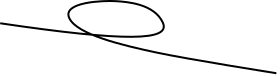
\includegraphics[width=.3\textwidth]{img/ptolemaeus_mars.pdf}
        \end{center}
    \item[Modelle]
        \begin{itemize}
            \item \textsc{Ptolemäus:}
                \begin{itemize}
                    \item Geozentrisch (Erde im Zentrum)
                    \item Planeten auf Epizykelbahnen
                \end{itemize}
            \item \textsc{Kopernikus:}
                \begin{itemize}
                    \item Heliozentrisch (Sonne im Zentrum)
                    \item \emph{Kreisbahnen}
                \end{itemize}
        \end{itemize}
    \item[Enscheidung] z. B. Planetenphasen der inneren Planeten\\
        $\Rightarrow$ Kopernisches Weltbild
\end{description}
\begin{itemize}
    \item \textsc{Kepler:} Messung d. Marsbahnen (T. \textsc{Brahe})\\
          $\Rightarrow$ \textsc{Kepler}'sche Gesetze (empirisch)
          \begin{enumerate}
              \item Ellipsen, Sonne in einem Brennpunkt
              \item Flächensatz $\Leftrightarrow$ Drehimpulserhaltung \\
                    Radiusvektoren überstreichen in gleicher Zeit gleiche Flächen,\\
                    d. h. Flächengeschwindigkeit = $\mathbf{const}$
              \item Umlaufzeiten/Abstände ($a$: Halbachse, $T$: Umlaufzeit)
                      \[ \frac{a^3}{T^2} \sim \mathbf{const} \]
          \end{enumerate}
\end{itemize}

\section{\textsc{Newton}'sche Mechanik}
\subsection{\textsc{Newton}'sche Axiome}
\begin{enumerate}[(i)]
    \item Trägheitsgesetz (Masse konstant, vergl. spezielle Relativitätstheorie):
        \begin{equation}
            \vec p = m \vec v = m \dot{\vec{r}} = m \frac{d}{dt} \vec r
            \label{eq:newton1}
        \end{equation}
    \item Impulsänderung durch Krafteinwirkung:
        \begin{equation}
            \frac{d}{dt} \vec p = \dot{\vec p} = \vec F = m \ddot{\vec r} = m \frac{d^2}{dt^2} \vec r = m \vec a
            \label{eq:newton2}
        \end{equation}
    \item Actio = Reactio:
        \begin{equation}
            \vec F_{ik} = -\vec F_{ki}
            \label{eq:newton3}
        \end{equation}
\end{enumerate}

\subsection{\textsc{Newton}'sche Gravitationsgesetze}
\noindent Formulierung für 2 Punktvektoren $m_1, m_2$
\paragraph{Skizze}
\begin{center}
        \begin{tikzpicture}[vector/.style={->}, >=stealth, auto]
            \coordinate [label=right:{$(0,0)$ Ursprung}] (O) at (0,0);
            \coordinate [label=above:$m_1$] (m1) at (0,2);
            \coordinate [label=above:$m_2$] (m2) at (2.2,2);

            \foreach \point in {O,m1,m2}
                \fill (\point) circle (2pt);
            \draw[vector] (O) -- (m1) node[align=center, midway] {$\vec r_1$};
            \draw[vector] (O) -- (m2) node[swap, align=center, midway] {$\vec r_2$};
            \draw[vector] (m1) -- (m2) node[align=center, midway] {$\vec r$};
        \end{tikzpicture}
        \begin{minipage}[b]{0.3\textwidth}
            \begin{align*}
                \vec r &= \vec r_1 - \vec r_2 \\
                |\vec r| &= r\\
                m &= m_1 + m_2
            \end{align*}
        \end{minipage}
\end{center}

\begin{equation}
    \boxed{\vec F = -\frac{G m_1 m_2 \vec r}{r^3}}
\end{equation}

\noindent $G$: \textsc{Newton}'sche Gravitationskonstante (vgl. \textsc{Einstein}'sche Gravitationskonstante $\kappa$)\\[0.5em]
\noindent Zweikörperproblem: Erhaltungsgrößen; Mit \autoref{eq:newton2} und \autoref{eq:newton3}:
\begin{equation}
    \boxed{m_1 \ddot \vec{r}_1 = \frac{G m_1 m_2 \vec r}{r^3},\qquad m_2 \ddot \vec{r}_2 = -\frac{G m_1 m_2 \vec r}{r^3}}
    \label{eq:newton_two_body}
\end{equation}

\begin{description}
    \item[Addition \autoref{eq:newton_two_body}]
        \begin{align*}
            m_1\vec{r}_1 + m_2\vec{r}_2 &= \frac{d^2}{dt^2} (m_1 \vec{r}_1 + m_2 \vec{r}_2) \\
                                      0 &= \frac{d^2}{dt^2} (m_1 \vec{r}_1 + m_2 \vec{r}_2)
        \end{align*}
        Differentialgleichung 2. Ordnung in der Zeit: $\int \cdots dt$
        \[ \Rightarrow \frac{d}{dt} (m_1 \vec{r}_1 + m_2 \vec{r}_2) = \vec{C}_{1+2} = \vec{p}_1 + \vec{p}_2 = \vec{p}_{\text{ges}} \]
        3 Konstanten $\rightarrow$ Impulserhaltung
        \[ \Rightarrow (m_1 \vec{r}_1 + m_2 \vec{r}_2) = \vec{C}_1 + \vec{C}_2 \]
        3 Konstanten $\rightarrow$ Schwerpunktsatz
    \item[Subtraktion \autoref{eq:newton_two_body}]
        \begin{align*}
            -\frac{G m_1 m_2 \vec r}{i m_2 r^3} - \frac{G m_1 m_2 \vec r}{m_1 r^3} &= \frac{\cancel{m_2} \ddot \vec{r}_2}{\cancel{m_2}} - \frac{\cancel{m_1} \ddot \vec{r}_1}{\cancel{m_1}} \\
            \ddot \vec{r} = - \frac{G \vec r}{r^3} m && \text{d.h. $\ddot \vec{r} \| \vec r$ (Zentralkraft)} \tag{$| \vec r \times$}\\
            \vec r \times \ddot \vec{r} = - \frac{Gm}{r^3} \underbrace{\vec r \times \vec r}_{= \vec 0} \\
            \frac{d}{dt} \left(\vec r \times \dot{\vec{r}}\right) = \vec 0
        \end{align*}
        Differentialgleichung 1. Ordnung in der Zeit\\[1em]
        \color{OliveGreen}
        \textbf{Nebenrechnung:}
        \[ \frac{d}{dt} (\vec r \times \dot{\vec{r}}) = \underbrace{\dot{\vec{r}} \times \dot{\vec{r}}}_{= \vec 0} + \vec r \times \ddot \vec{r} \tag{Produktregel} \]
        \color{black}
        \textbf{Lösung:} $\int \cdots dt$
        \begin{align*}
            \vec r \times \dot{\vec{r}}             &= \vec{C}_3 \\
            \vec r \times \frac{m}{m} \dot{\vec{r}} &= \frac{1}{m} (\vec r \times \underbrace{m \vec v}_{\vec p})\\
                                                    &= \frac{1}{m} \underbrace{(\vec r \times \vec p)}_{\vec L} \tag{$\vec L$: Drehimpuls}
        \end{align*}
        $\Leftrightarrow$ Drehimpulserhaltung\\
        $\Leftrightarrow \dot{\vec{L}} = 0$\\
        $\Leftrightarrow \dot{\vec{L}} = \textbf{const}$\\
        Aus der Addition von \autoref{eq:newton_two_body} mit $\vec{r}_2$ bzw. $\vec{r}_1$ folgt:
        \begin{align*}
            m_1 \langle\dot{\vec{r}}_1, \ddot{\vec{r}}_1\rangle + m_2 \langle\dot{\vec{r}}_2, \ddot{\vec{r}}_2\rangle 
                &= \frac{Gm_1m_2}{r^3} \left(\langle\vec{r}, \vec{r}_1\rangle - \langle\vec{r}, \vec{r}_2\rangle\right)\\
                &= \frac{Gm_1m_2}{r^3} (\underbrace{\langle\vec{r}_2 - \vec{r}_1, \vec{r}_1\rangle - \langle\vec{r}_2 - \vec{r}_1, \vec{r}_2\rangle}_{?})\\
        \end{align*}
        \color{OliveGreen}
        \textbf{Nebenrechnung:} $i \in {1,2}$
        \[\frac{d}{dt}\dot{\vec{r}}_i^2 = \langle2\dot{\vec{r}}_i, \ddot{\vec{r}}_i\rangle \tag{Kettenregel}\]
        \color{black}
        \begin{align*}
            \frac{d}{dt}(\vec{r}_2 - \vec{r}_1) &= \langle2(\vec{r}_2 - \vec{r}_1), \dot{\vec{r}}_2 - \vec{r}_1\rangle\\ 
                                                &= -2 \left(\langle(\vec{r}_2 - \vec{r}_1), \dot{\vec{r}}_1\rangle - \langle(\vec{r}_2 - \vec{r}_1), \vec{r}_2\rangle\right)\\
                                                &= \frac{d}{dt} r^2
        \end{align*}
        Damit gilt:
        \begin{align*}
            \frac{d}{dt} \sum\limits_{i = 1}^{2} \frac{m_i}{2} \dot r^2 &= -\frac{Gm_1m_2}{2r^3} \frac{d}{dt} r^2\\
                                                                        &= -\frac{Gm_1m_2}{2r^1} \underbrace{\frac{1}{r} \frac{d}{dt} r^2}_{?} \tag{skalare Gleichung}
        \end{align*}
        \color{OliveGreen}
        \textbf{Nebenrechnung:}
        \begin{align}
            \frac{1}{r} \frac{d}{dt} r^2            &= \frac{1}{\cancel{r}} 2 \cancel{r} \dot{r} = 2 \dot{r} \label{eq:newton_nr_1}\\
            \frac{d}{dt} \left(\frac{1}{r}\right)   &= \frac{1}{r^2} 2 \dot{r} \Leftrightarrow \dot{r} = -r^2 \frac{d}{dt} \left(\frac{1}{r}\right) \label{eq:newton_nr_2}\\
            \text{\autoref{eq:newton_nr_1} + \autoref{eq:newton_nr_2}:}\quad \frac{1}{r} \frac{d}{dt} r^2 &= -2r^2 \frac{d}{dt}\left(\frac{1}{r}\right)
        \end{align}
        \color{black}
        Daris folgt: Differentialgleichungssystem
        \begin{align*}
            \frac{d}{dt}\left(\sum\limits_{i=1}^{2} \frac{m_i}{2} \dot r^2_i\right) &= \cancel{-}\frac{Gm_1m_2}{\cancel{2r^2}} \left[\cancel{-}\cancel{2r^2}\frac{d}{dt} \left(\frac{1}{r}\right)\right]\\
                                &= Gm_1m_2 \frac{d}{dt} \left(\frac{1}{r}\right)
        \end{align*}
        \begin{align*}
            \Rightarrow \frac{d}{dt} \left(\sum_{i = 1}^{2} \frac{m_i}{2} r_i^2 - \frac{Gm_1m_2}{r}\right) &= 0 \tag{s. dd}\\
            \underbrace{\sum\limits_{i = 1}^2 \frac{m_i}{2} \dot{r}_i^2}_{E_{\text{kin}}} - \underbrace{\frac{Gm_1m_2}{r}}_{E_{\text{pot}}} &= C_4 = E_{\text{ges}}
        \end{align*}   
        1 Konstante $\Rightarrow$ Energiesatz \\
        Phasenraum: $(2 \cdot 6) = 12 \rightarrow 10$ Integrale der Bewegung\\
        $\Rightarrow 2$ Division $\rightarrow$ Bahnebene $\bot\ \vec L = \mathbf{const}$
\end{description}

\section{2-Körperproblem -- Kepler Gesetze}

\section{Bemerkungen zu Störeffekten}
\section{Virialsatz}

\part{Planeten}
\chapter{Physikalische Eigenschaften des Sonnensystems}
\section{Stabilität der Atmosphäre}
\section{Energiehaushalt und Atmosphärentemperatur}


\section{Stabilität eines Mondes (Planeten) gegenüber Störungen durch 
         Gezeitenkräfte}
\paragraph{Skizze}
\begin{center}
    \begin{tikzpicture}
        \draw (0,0) circle (1.5) node {$\times$};
        \node [below] at (0,-1.5) {Planet $M$};
        \draw (8,0) circle (1.0) node {$\times$};
        \node [below] at (8,-1.5) {Mond $m$};
        \draw [dashed] (8, -1.5) -- (8, 1.5);
        \draw [|-|] (0,-0.5) -- (8,-0.5) node [pos=0.5, above] {$r$};
        \draw [|-|] (7.5,-1) -- (8.5,-1) node [pos=0.7, above] {$R$};
        \draw (8, 0) -- (9, 0) node [pos=0.5, below] {$R$};
        \node [above] at (7.5,0) {$1$};
        \node at (7.5,0) {$\bullet$};
        \node [above] at (8.5,0) {$2$};
        \node at (8.5,0) {$\bullet$};
    \end{tikzpicture}
\end{center}
\begin{align*}
    r_1 &= r - \frac{R}{2} \\
    r_2 &= r + \frac{R}{2}
\end{align*}

\paragraph{Betrachte}
\begin{enumerate}[i)]
    \item Gravitationskraft: "`Hälften"'
        \[ F_M = - G \frac{m}{2} \frac{m}{2} \frac{1}{R^2} \]
        $\rightarrow$ bestimmt den "`Zusammenhalt des Mondes"'
        (Vernachlässigung der Festkörpereigenschaften!!!)
    \item Unterschiedliche Gravitationskräfte eines 2. Körpers (Planet) auf
        die beiden "`Hälften"'
        \begin{align*}
            F_1 &= -G M \frac{m}{2} \frac{1}{r_1^2} = \frac{GMm}{2} \frac{1}{\left(r-\frac{R}{2}\right)^2}
            F_2 &= -G M \frac{m}{2} \frac{1}{r_2^2} = \frac{GMm}{2} \frac{1}{\left(r+\frac{R}{2}\right)^2}
        \end{align*}
\end{enumerate}

\begin{definition}
    Gezeitenkraft
    \[ F_{\mathrm{Gez}} = F_1 - F_2 = - \frac{GMm}{2} \left(\frac{1}{\left(r-\frac{R}{2}\right)^2} - \frac{1}{\left(r+\frac{R}{2}\right)^2}\right) \]
\end{definition}

\paragraph{Allgemein} $r \gg R$ (gilt \emph{nicht} für enge Doppelsterne)

Reihenentwicklung:
\[ \frac{1}{x^2} = \frac{1}{x_0^2} - \frac{2}{x_0^3} (x-x_0) + 0\]
\begin{align*}
    \frac{1}{\left(r - \frac{R}{2}\right)^2} &= \frac{1}{r^2} + \frac{1}{r^3} R\\
    \frac{1}{\left(r + \frac{R}{2}\right)^2} &= \frac{1}{r^2} - \frac{1}{r^3} R\\
    \Rightarrow F_{\mathrm{Gez}} &= -\frac{GMm}{2} \left(\frac{R}{r^3} + \frac{R}{r^3}\right) = G M m \frac{R}{r^3}
\end{align*}

\paragraph{Bedingung} Stabilität: $|F_m| > |F_{\mathrm{Gez}}|$
\[ \frac{4M}{m} < \left(\frac{r}{R}\right)^3 \Leftrightarrow \frac{m}{4M} > \left(\frac{R}{r}\right)^3 \]
\begin{align*}
    M &= \bar \rho_{\mathrm{Pl}} \cdot \frac{4}{3} \pi R_{\mathrm{m}}^3 & m &= \bar \rho_{\mathrm{Pl}} \cdot \frac{4}{3} \pi R^3
\end{align*}
\[ \Rightarrow r > \sqrt[3]{4 \frac{\bar \rho_{\mathrm{Pl}}}{\bar \rho_{m}}} \cdot R_{\mathrm{Pl}} \]
Genaure Rechnung liefert: \textsc{Roche}-Grenze
\[ \Rightarrow r > \sqrt[3]{\frac{\bar \rho_{\mathrm{Pl}}}{\bar \rho_{m}}} \cdot 2.44 \cdot R_{\mathrm{Pl}} \]

\section{Bedingungen für Planetenentstehung}
Entstehung aus Staub-/Gasscheiben von jungen Sternen $\rightarrow$ Beispiel: $\beta$ Pic

\paragraph{Szenario} Sonnensystem
\begin{itemize}
    \item Sternwind $T$ im inneren Sonnensystem hoch
    \item Sternwind $T$ im äußeren Sonnensystem niedrig \\
        $\Rightarrow$ Akkredition von Restgas
    \item Ausdünnung der Scheibe nach außen
    \item kleine Gesteinsplaneten innen
    \item große Planeten mittig
    \item Gasplaneten weiter außen
    \item Kometen ganz außen
\end{itemize}

\paragraph{Prolem} Neue Planetenklasse

``Hot Jupiter'': sehr massereiche Gasplaneten nah am Stern

$\Rightarrow$ konkurierende Entstehungstheorien:
\begin{itemize}
    \item \framebox{in situ}
    \item \framebox{Migration}
\end{itemize}

\chapter{Extrasolare Planeten}
\section{Beobachtungsmethoden}
\subsection{Radialgeschwindigkeitsmethode}
\subsection{Astronomie}

\subsection{Transitmethode}
\paragraph{Prinzip} Bedeckung des Sterns des Planeten\\
$\Rightarrow$ "`Einbruch"' in der Lichtkurve

\paragraph{Problem} Auswahleffekt $i$ im Bereich von $90\degree$
\paragraph{Vorteil} sehr kleine Planeten beobachtbar
\paragraph{Beispiel} HD209458 b
\begin{align*}
    i &= 87.1\degree & R_{\Pl} &= 1.27\,R_{\jupiter}
\end{align*}
\paragraph{RV-Messung} $M_{\Pl} \cdot \sin i = 0.63\, M_{\jupiter}$
\begin{align*}
    \Rightarrow M_\Pl &= \frac{0.63}{0.9987}\,M_{\jupiter} & M_{\jupiter} &= 1.197 \cdot 10^{30}\,\gram \\
    R_\Pl &= 1.27\,R_{\jupiter} = 9.067 \cdot 10^{7}\,\metre \\
    \Rightarrow \rho_\Pl &= \frac{M_\Pl}{\frac{4}{3} \pi R_\Pl^3} \approx 0.38\,\frac{\gram}{\metre^3} \tag*{$\rightarrow$ weniger dicht als Saturn}
\end{align*}

\paragraph{Satelliten-Missionen}
\begin{itemize}
    \item COROT
    \item Kepler
    \item PLATO (2024)
\end{itemize}

\subsection{Microlensing Methode}
\paragraph{Prinzip} Charakteristische Lichtkurve durch einen
Gravitationslinsenstern mit Planet

\paragraph{Situation}
\begin{center}
    \begin{minipage}[h]{0.5\textwidth}
        \begin{tikzpicture}
            \node (Quelle) at (0,4) {$\circledast$};
            \node [above] at (Quelle) {Quelle (Stern)};
            \node (Linse) at (0,2) {$\bullet$};
            \node [right,xshift=0.5cm] at (Linse) {Linse};
            \coordinate (Beob) at (0,0);

            \node at (-0.25,2) {$\circ$};
            \node at (1,4) {$\circledast$};
            \node at (-0.5,4) {$\circledast$};
            \node at (-1,4) {$\circledast$};

            \draw plot[smooth,tension=0.5] coordinates{(1,4) (0.25,2) (Beob)};
            \draw (-0.5, 4) -- (-0.25,2);
            \draw (-1, 4) -- (-0.25,2);
            \draw (-0.25,2) -- (0,0);
        \end{tikzpicture}
    \end{minipage}
    \begin{minipage}[h]{0.4\textwidth}
         \begin{tikzpicture}
             \draw [->] (0,0) -- (4,0);
             \draw [->] (0,0) -- (0,2);
             \draw plot [smooth] coordinates{(0.5,0.5) (1.2,0.6) (1.3,1.8)
                                             (1.5,1.5) (1.7,1.8) (2,1.55)
                                             (2.2,1.8) (3,0.75) (3.8, 0.5)};
             \node at (2,2.5) {Lichtkurve};
         \end{tikzpicture}
    \end{minipage}
\end{center}

\subsubsection{Gravitationslinsen-Gleichung}
\paragraph{Annahme} Dünne Gravitationslinsen-Approxmation \\
$\Rightarrow$ lensing effect durch:
\begin{itemize}
    \item einzelne Materiensammlung
    \item in einer bestimmten Entfernung
\end{itemize}

\paragraph{Skizze}
\begin{center}
    \begin{tikzpicture}
        \coordinate (L) at (0,5);
        \node at (L) {$\bullet$};
        \node [anchor=south west] at (L) {$L$};
        \coordinate (S) at (3,7);
        \node at (S) {$\bullet$};
        \node [above] at (S) {$S$};
        \coordinate (S1) at (4.5,7);
        \node at (S1) {$\bullet$};
        \node [above] at (S1) {$S_1$};

        \draw [|-|] (-1.2,1) -- (-1.2,7) node [left,pos=0.5] {$D_S$};
        \draw [|-|] (-0.2,1) -- (-0.2,5) node [left,pos=0.5] {$D_L$};
        \draw [|-|] (-0.2,5) -- (-0.2,7) node [left,pos=0.5] {$D_{LS}$};

        \draw (60:0.5) -- (0,0) -- (120:0.5); 
        \draw (0,0) ++ (60:0.3) arc (60:120:0.3);
        \draw (0,1) -- (0,7);
        \draw (0,1) -- (S);
        \draw (0,1) -- (S1);
        \draw (0,7) -- (6,7) node [right] {Ebene der Quelle};
        \draw (L) -- (6,5) node [right] {Ebene der Linse};
        \draw (3,5) -- (S);
        \node at (1,5) [below] {$\xi$};
        \node at (1.5,7) [below] {$\eta$};
        \node at (3.75,7) [below] {$\varphi$};

        \draw (0,4.5) arc (270:360:0.5);
        \node at (0.2,4.8) {$\cdot$};
        \draw (2.5, 5) arc (180:90:0.5);
        \node at (2.8,5.2) {$\cdot$};
        \draw (3, 5) ++ (53.13:1.2) arc (53.13:90:1.2);
        \node at (3.3, 5.8) {$\tilde \alpha$};
        \draw [blue] (0,1) ++ (53.13:2) arc (53.13:90:2);
        \node at (0.5,2.5) {\color{blue} $\theta$};
        \draw [red] (0,1) ++ (63.43:3) arc (63.43:90:3);
        \node at (0.615, 3.4) {\color{red} $\beta$};
        \draw [green] (0,1) ++ (53.13:3) arc (53.13:63.43:3);
        \node at (1.4, 3.3) {\color{green} $\alpha$};
    \end{tikzpicture}
\end{center}

\begin{align*}
    \theta &= \beta + \alpha (\theta) \\
    D_S &= D_L + D_{LS}
\end{align*}o

\paragraph{Kleine Winkel}
\begin{align*}
    \beta &\approx \tan \beta = \frac{\nu}{D_S} \\
    \theta &\approx \tan \theta = \frac{\xi}{D_L} = \frac{\nu + \varphi}{D_S} > \beta + \alpha \\
    \alpha &\approx \frac{\varphi}{D_S} \Rightarrow \varphi = \alpha D_S = \tilde \alpha D_{LS}
\end{align*}

\paragraph{Annahme} local -- \textsc{Minkowski}-Raum (flach)
\[ \Rightarrow \boxed{\alpha = \left(\frac{D_{LS}}{D_S}\right) \tilde \alpha} \]

\begin{definition}
    \textbf{Ablenkungswinkel $\tilde \alpha$:} Lichtablenkung: Beschreibung durch
    "`Prismeneffekt"' \\
    $\hookrightarrow$ effektiven "`Brechungsindex"': $n = 1 + \frac{2}{c^2} \Phi$
\end{definition}

\paragraph{Gravitationspotential} $\Phi < 0$ 

\begin{align*}
    \tilde \alpha &= -\int \nabla_\bot n\ ds = -\int \nabla_\bot (1 + \frac{2}{c^2} \Phi)\ ds \\
                  &= -\frac{2}{c^2} \int \nabla_\bot \Phi\ ds
\end{align*}

\paragraph{Situation} Punktmasse $M$

\paragraph{Annahme} kleine Störung $\Rightarrow$ Integration entlang des ungestörten Weges \\
$b$: Impaktparameter

\begin{center}
    \begin{tikzpicture}
        \coordinate (S1) at (0,0);
        \coordinate (S) at (-1,0);
        \coordinate (M) at (-0.7,2);
        \node at (0,2) {$\bullet$};
        \node at (M) {$\bullet$};
        \draw [yshift=4.5cm] (240:0.5) -- (0,0) -- (300:0.5);
        \draw [yshift=4.5cm] (0,0) ++ (240:0.3) arc (240:300:0.3);
        \draw (S1) -- (0,4);
        \draw [dotted] plot[smooth,tension=0.5] coordinates{(0,4) (-0.7/2,2) (S)};
        \draw (M) -- (0,2) node [pos=0.5,above] {$b$};
        \draw (-0.25,2) arc (180:270:0.25);
        \node at (-0.1,1.9) {$\cdot$};
        \node [right] at (0,1.625) {$z$};
        \draw (M) -- (0,1.25) node [pos=0.5,anchor=north east] {$r$};
        \draw (-0.25,2) arc (180:270:0.25);
    \end{tikzpicture}
\end{center}

\paragraph{Bereich größter Annäherung}
\begin{align*}
    r &= \sqrt{b^2 + z^2} \\
    \Delta z &\approx \pm b \\
    \Phi(r) &= -\frac{GM}{r} = -\frac{GM}{\sqrt{b^2 + z^2}} = \Phi(b,z) \\
    \Rightarrow \nabla_\bot \Phi &= \frac{\partial}{\partial b} \Phi(b,z) \\
    \Rightarrow \tilde \alpha &= -\frac{2}{c^2} \int\limits_{-\infty}^{\infty} \frac{\partial}{\partial b} \left(-\frac{GM}{\sqrt{z^2 + b^2}}\right)\ dz \\
    &= \frac{2GM}{c^2} b \int\limits_{-\infty}^{\infty} \frac{1}{(b^2 + z^2)^{\frac{3}{2}}}\ dz
\end{align*}

Substitiution: $x := \dfrac{z}{b} \Rightarrow \dfrac{dx}{dz} = \dfrac{1}{b} \Rightarrow dz = b\ dx$

\begin{align*}
    \Rightarrow \tilde \alpha &= \frac{2GMb^2}{c^2} \underbrace{\int\limits_{-\infty}^{\infty} \frac{dx}{(1 + x^2)^{\frac{3}{2}}}}_{= 2} \cdot \left(\frac{1}{b^3}\right)\ dx \\
    &= \frac{2GM}{c^2b} \cdot 2 = \frac{4GM}{c^2 \cdot b} = \tilde \alpha
\end{align*}

\paragraph{Vergleich} Schwarzschildradius
\paragraph{"`Motivation"'} $v_{\mathrm{esc}} (R_S) = c$
\[ c = \sqrt{\frac{2GM}{R_S}} \Rightarrow \boxed{R_S = \frac{2GM}{c^2}} \]
$\Rightarrow$ \textbf{Ablenkwinkel:} $\boxed{\tilde \alpha = 2\left(\dfrac{R_S}{b}\right)}$

\paragraph{Beispiel} Ablenkung am Sonnenrand $\boxed{b = R_{\astrosun}}$
\[ \alpha = \frac{4GM_{\astrosun}}{c^2 R_{\astrosun}} = 1.7\arcsecond \]
\paragraph{Beobachtung} \textsc{Eddington} (1919): $20\,\%$ Bestätigung

\subsubsection{Einstein-Ring}
\paragraph{Bedingung} Quelle -- Linse -- Beobachter
\[ \beta{\Theta_E} = 0 \Rightarrow \underset{\mathclap{\text{Einstein-Radius}}}{\boxed{\Theta_E = \sqrt{\frac{D_{LS}}{D_S D_L} \frac{GM(\Theta_E)}{c^2}}}} \]

\subsection{Direkte Beobachtung}

\chapter[Doppelsterne]{Doppelsterne (DS)}
\section{Klassen von DS}
\section{Roche-Lobe-Massentransfer}

\part{Astronomische Beobachtungsgrößen}
\chapter{Astronomische Spektroskopie}
\section[Astronomische Helligskeitsysteme]{Astronomische Helligskeitsysteme (Bsp. Sterne)}
\section{Filtersysteme}

\section{Interstellare Verfärbung}
\paragraph{Ursache} Interstellare Materie / Speziell: Staubteilchen

% TODO Graphic

\begin{itemize}
    \item Re-Emission bei $T_{\text{Staub}} \sim 10^2\,\kelvin \rightarrow$ IR ("`Rötung"')
    \item isotrope Streuung (kleine Staubteilchen) $\rightarrow$ aus der Richtung gestreut
\end{itemize}

\paragraph{Verfärbung} Schwächung der scheinbaren Helligkeit
\[ \Delta m_{\lambda} = A_{\lambda} \sim \frac{1}{\lambda} \]

\paragraph{Beschreibung} Farbexzess $E$
\[ E_{B-V} = \underset{\text{beobachtet}}{(B-V)_{\mathrm{obs}}} - \underbrace{(B-V)_0}_{\text{Eigenfarbe des Objekts}} = A_B - A_V \]

Empirischer Zusammenhang: $A_V \approx (3.0 \pm 0.2)\,E_{B-V}$

\section{Bolometrische Korrektur (B.C.)}
! Sterne !

% TODO Graphic

\[ \boxed{B.C. = m_v - m_{\mathrm{bol}}} \]

\framebox{Korrekturen werden aus Sternatmosphärenmodellen abgeleitet.}

\section{Susammenhang: Absolute bolometrische Helligkeit $\leftrightarrow$ Leuchtkraft}
\[ L_* = 4 \pi R_*^2 F_* \]

\paragraph{Annahme} keine Verfärbung

\begin{align*}
    r = 10\,\parsec{:}\ f(10\,\parsec) &= F_*\left(\frac{R_*}{10\,\parsec}\right)^2 = \frac{L_*}{4 \pi \cancel{R_*^2}} \left(\frac{\cancel{R_*}}{10\,\parsec}\right)^2 \\
    m_{\mathrm{bol}} (10\,\parsec) = M_{\mathrm{bol}}^{*} &= -2.5 \log f (10\,\parsec) + C \\
                                                          &= -2.5 \log \left(\frac{f_* R_*^2}{(10\,\parsec)^2}\right) \\
                                                          &= -2.5 \log (L_*) + 2.5 \cancel{\log(4\pi)} + \cancel{5} \underset{\approx 1}{\cancel{\log(10\,\parsec)}} + \cancel{C}
\end{align*}

Analog für Sonne:
\begin{align*}
    M_{\mathrm{bol}}^{\astrosun} &= -2.5 \log L_{\astrosun} + 2.5 \cancel{\log(4\pi)} + \cancel{5} + \cancel{C} \\
    \Rightarrow M_{\mathrm{bol}}^* - M_{\mathrm{bol}}^{\astrosun} &= -2.5 \log\left(\frac{L_*}{L_{\astrosun}}\right) \\
    M_{\mathrm{bol}}^{\astrosun} &= 4.72\magnitude \\
    M_{\mathrm{bol}}^* &= 4.72\magnitude - 2.5\magnitude \log\left(\frac{L_*}{L_{\astrosun}}\right)
\end{align*}

\section{Spektralklassifikation und HR-Diagramm}
\paragraph{Prinzip} Spektren werden in Klassen zusammengefasst

\paragraph{Umrechnung nach Havard-Sequenz} $\rightarrow T_{\mathrm{eff}}$

\[ O - B - A - F - G - K - \overbracket{M - L - T - Y}^{\mathclap{\text{Braune Zwerge}}} \]

% TODO HRD

\paragraph{Problem} HRD ist bezüglich Spektralklassen nicht eindeutig $\rightarrow$ Leuchtkraftklassen

\subsubsection{Masse-Leuchtkraftbezeichnung auf der Hauptreihe}
\[ \log\left(\frac{L_*}{L_{\astrosun}}\right) \sim \log \left(\frac{M_*}{M_{\astrosun}}\right) \]

\[
    \boxed{\log\left(\frac{L_*}{L_{\astrosun}}\right) = \begin{cases}
        2 \log \left(\frac{M_*}{M_{\astrosun}}\right) - 0.4, & \text{sonst} \\
        4 \log \left(\frac{M_*}{M_{\astrosun}}\right), & \text{für $M_* > 0.6 M_{\astrosun}$} \\
    \end{cases}}
\]

% TODO Graph

\subsubsection{Fundamentale Sternparameter}

\[ \underbrace{\underbrace{L_*, T_*}_{R_*}, M_*}_{\text{Oberflächenbeschleunigung $g_* = \dfrac{GM_*}{R_*^2}$}}, \underset{\text{dynamische Elemente (Elementzusammensetzung -- Metallizität)}}{\{\epsilon_i\}} \]

% next chapter

\chapter{Entfernungsbestimmungsmethoden}
\section{Laufzeitmethoden}
\section{Geometrische Methode}
\subsection{Trigonometrische Parallaxe}
\subsection{Sternstromparallaxe}
\subsection{Säkuläre Parallaxe}
\subsection{Durchmessermethode}
\section{Photometrische Methode}
\subsection{FH-Diagramm Parallaxe}
\subsection{Spektroskopische Parallaxe}

\subsection{Cepheidenmethode}
\subsection[Standardkerzen]{Standardkerzen (Super Novae/Novae)}
\subsection{Rotverschiebungsmethode}
\subsection{Entfernungsleiter: Vermessung des Universums}

\part{Galaxis -- Die Milchstraße}
\chapter{Bau der Milchstraße}
\chapter{Kinematik}
\section{Rotationskurve}
\section{Diferentielle Rotation der Galaxis}

\end{document}
